% this file is called up by thesis.tex
% content in this file will be fed into the main document

\chapter{Rendering techniques} % top level followed by section, subsection

\graphicspath{{techniques/figures/}}

% ----------------------- contents from here ------------------------

Output from particle base simulations is a list of particles containing positions. It can also contain additional parameters - for example PhysX fluid simulation returns velocity, lifetime and density, in addition to position, for each particle. 

Traditionally triangle meshes are used for rendering objects. Using this approach requires constructing fluid's triangle mesh for given particle positions. This method is called isosurface extraction and will be described in section~\ref{sec:isosurfaceextraction}.
Another possibility is to render each particle as a point (or a billboard in general) with opacity so when large amount of particles is rendered the result would give illusion of a smooth surface. Such technique has one major drawback - it does not produces surface preventing us from adding effects of reflection and refraction.
Similar technique is to extract visible surface by rendering each particle as a sphere into depth buffer. This will be described in section~\ref{sec:screen_space}.

\section{Screen space} \label{sec:screen_space}
\figuremacroW{screen_space}{Screen Space Fluid Rendering}{The figure shows high level overview of the method, taken from \cite{Green2010}}{0.7}
As mentioned before this approach extracts visible surface by rendering each particle into depth buffer. High level overview ot this method is presented on figure~\ref{screen_space} and consists of following steps \cite{laanSainz2009}: rendering depth texture (section~\ref{sec:surfacedepth}) and thickness textures (section~\ref{sec:thickness}), depth smoothing (section~\ref{sec:smoothing}) and assembling fluid surface with rest of the scene (section~\ref{sec:screenspace_rendering}).

\subsection{Surface depth} \label{sec:surfacedepth}
To obtain fluid's surface visible from the viewpoint of camera each particle is rendered as a sphere into depth texture (figure~\ref{sphere_depth}). At each pixel only closest value is kept using hardware depth test. 
\figuremacroW{sphere_depth}{Particles rendered as spheres into depth texture}{}{0.7}
In order to avoid rendering large amount of geometry each particle is rendered as a point sprite and it's depth is generated in fragment shader. This common technique speeds up rendering process significantly as well as improves quality of rendered spheres (as can be seen on figure~\ref{spheres}). Rendering spheres as point sprites is 10 to 100 times faster comparing to rendering them as triangle meshes (see table~\ref{sphere_speed_comp}).
\figuremacroW{spheres}{Spheres rendered with different methods}{1 - mesh with 128 triangles, 2 - mesh with 512 triangles, 3 - mesh with 2048 triangles, 4 - point sprite with normals generated in fragment shader}{0.5}
\begin{table}[htdp]
\caption[Comparision of sphere rendering methods]{\textbf{Comparison of sphere rendering methods}}
\centering
\begin{tabular}{cr} 
{\bf Method} & {\bf Frames per second} \\ 
\hline 
Mesh, 128 triangles & 20 \\
Mesh, 512 triangles & 6 \\
Mesh, 2048 triangles   & 1 \\
Point Sprites & 200 \\
\end{tabular}
\label{sphere_speed_comp}
\end{table}

\subsection{Smoothing} 
\label{sec:smoothing}
Although previous step produces surface, its quality is not sufficient. As can be seen on figure~\ref{spheres_no_smoothing} individual spheres can be seen giving fluid's surface unnatural appearance. To remove this artifact some kind of smoothing has to be applied. Section~\ref{sec:gaussiansmoothing} will describe Gaussian smoothing and section~\ref{sec:curvatureflowsmoothing} curvature flow smoothing.
\figuremacroW{spheres_no_smoothing}{Fluid surface rendered without smoothing phase}{Individual spheres can be seen, giving surface unnatural appearance}{0.7}

\subsubsection{Gaussian smoothing} \label{sec:gaussiansmoothing}
Most obvious way to smooth values in depth texture is to apply Gaussian filter. It's easy to implement and can be computed fast due to its linear separability. However this filter produces undesired effect of blending drops of fluid with background surfaces (see figure~\ref{gaussian_filter_img}). 
%\figuremacroW{gaussian_filter_img}{Fluid surface rendered with Gaussian smoothing}{it can be seen that different parts of fluid are blended together creating undesired effect of one big surface.}{0.7}
\begin{figure}[ht]
\begin{minipage}[b]{0.5\linewidth}
\centering
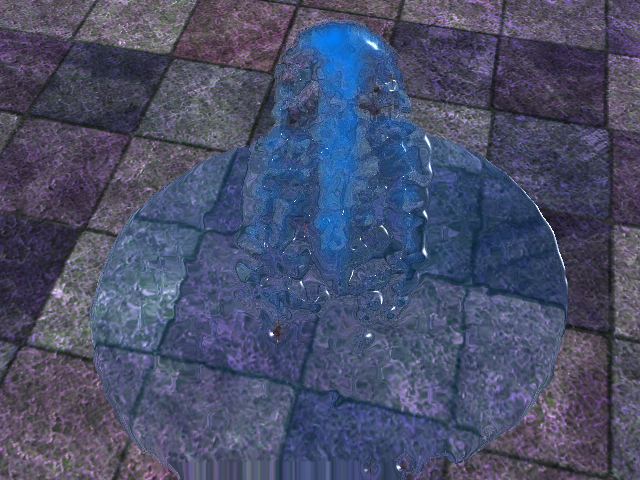
\includegraphics[width=1\textwidth]{nonbilateral_filter}
(a) Gaussian smoothing
\end{minipage}
\hspace{0.2cm}
\begin{minipage}[b]{0.5\linewidth}
\centering
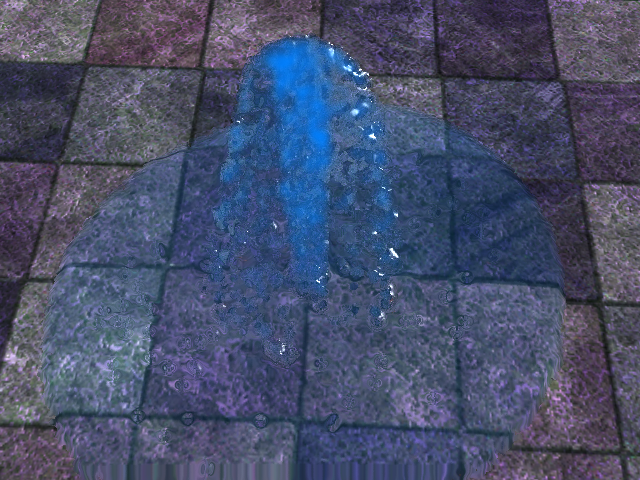
\includegraphics[width=1\textwidth]{bilateral_filter}
(b) Bilateral Gaussian smoothing
\end{minipage}
\caption{\textbf{Bilateral smoothing vs regular smoothing} - (a) Regular Gaussian smoothing it can be seen that surface of fountain is blended with fluid that lies on the ground, (b) bilateral filtering does not produce this undesired effect. }
\label{gaussian_filter_img}
\end{figure}
Thus edge-preserving filters (also called bilateral filters) needs to be used. Bilateral Gaussian filter is a modification that changes wages of pixels depending on difference between their tonal value $I(s)$ and tonal value of central pixel $I(s_0)$. This can be described by following formula (from~\cite{PhamVliet2005}): 
\begin{equation}
\label{bilateral_equation}
O(s_0) = \frac{\sum_{s \in S}f(s, s_0)I(s)}{\sum_{s \in S}f(s, s_0)}
\end{equation}
where 
\begin{equation}
\label{bilateral_weights_equation}
f(s, s_0) = g_s(s-s_0)g_t(I(s)-I(s_0))
\end{equation}
is the bilateral filter for the neighborhood around $s_0$, $g_s$ is a spatial weight, $g_t$ is a tonal weight and they both are Gaussian functions:
\begin{equation}
\label{bilateral_dist_equation}
g_s(s) = g(x, \sigma_S)g(y, \sigma_S)  \quad   g_t(I) = g(I, \sigma_t)
\end{equation}

As can be seen in equation~\ref{bilateral_weights_equation} only change in bilateral filter (in comparison to regular bilateral filter) is introduction of tonal weight $g_t$. This change makes filter space-variant - that means it can't be computed as a product of two one-dimensional filters ($g_s$ in equation~\ref{bilateral_dist_equation}). 
Computational complexity of space-variant filters is $O(Nm^d)$ comparing to only $O(Nmd)$ for space-invariant (d is image dimensionality, m is the size of filtering kernel and N is the number of pixels in the image). For smoothing fluid surface kernel with $m = 20$ must be used, which, when using bilateral filtering on 2 dimensional image, gives about 400 operations for each pixel. In comparison separable implementation requires only 40 operations. It turns out however that computing bilateral filter as if it was space-invariant gives good approximation for real time applications (see figure~\ref{bilateral_comp}). Approximation gives some artifacts but they are not visible when fluid is moving and other effects (reflection and refraction) are applied.

%\figuremacroW{bilateral_comp}{Comparision of normal bilateral filter with it's separable approximation}{Upper row presents images for bilateral filter and bottom row presents separable approximation.}{0.7}
\begin{figure}[ht]
\begin{minipage}[t]{0.5\linewidth}
\centering
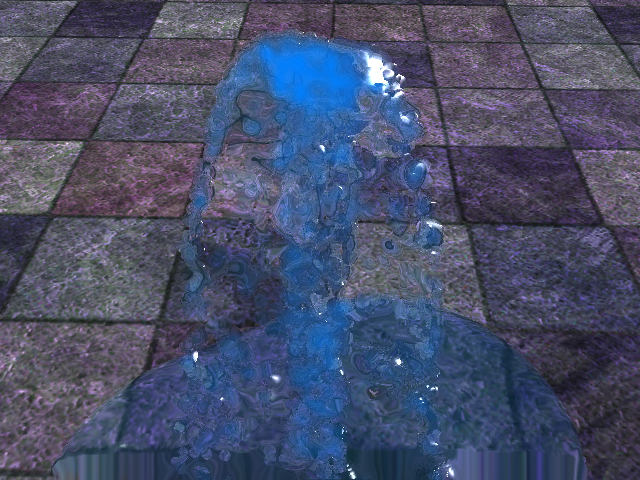
\includegraphics[width=1\textwidth]{cmp_bilateral}
(a) Bilateral Gaussian smoothing
\end{minipage}
\hspace{0.2cm}
\begin{minipage}[t]{0.5\linewidth}
\centering
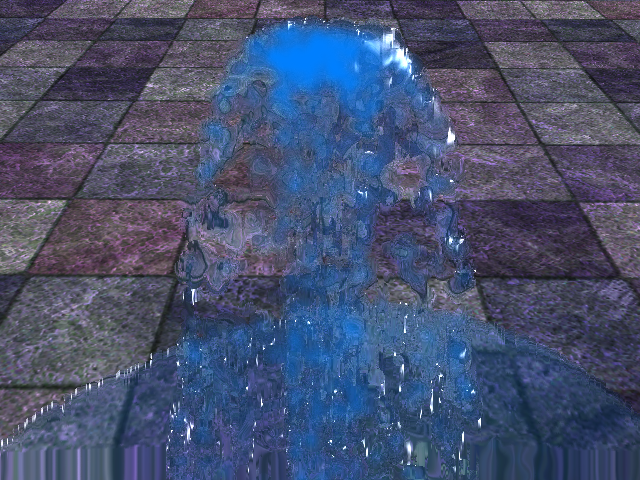
\includegraphics[width=1\textwidth]{cmp_bilateral_separable}
(b) Bilateral Gaussian smoothing computed as if it was separable
\end{minipage}
\caption{\textbf{Comparision of normal bilateral filter with it's separable approximation} -  Computing bilateral Gaussian filter as if it was separable produces some artifacts on edges (b), however they are not very disturbing.}
\label{bilateral_comp}
\end{figure}

Bilateral filter has some undesired effect when applied on z-buffer output. The problem is that depth values are not evenly distributed. This means that difference between two fragments depth values is dependent on their distance to the viewer. As can be seen on equation~\ref{bilateral_weights_equation} bilateral weights takes into account difference between depth values. As a result the further surface lies from camera the less edges are preserved (see figure~\ref{edge_preservation}). In that situation linear depth values have to be generated in fragment shader as described in section~\ref{sec:depth_buffer}. To produce linearly distributed depth values I am using equation~\ref{eq:linear_depth}.
\begin{figure}[ht]
\begin{minipage}[t]{0.5\linewidth}
\centering
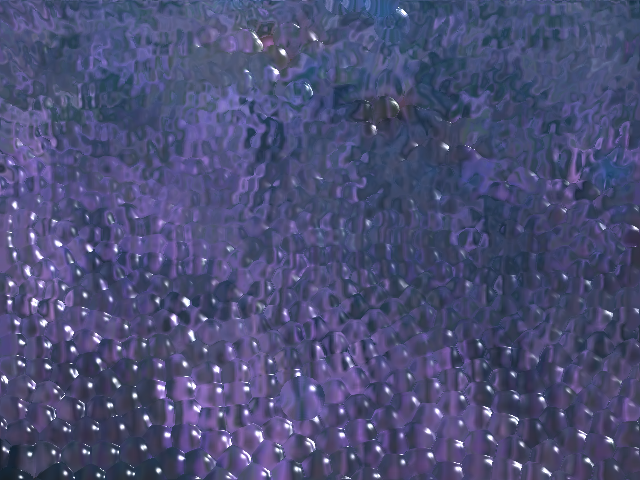
\includegraphics[width=1\textwidth]{gauss_fixed_close}
(a) Closer to camera
\end{minipage}
\hspace{0.2cm}
\begin{minipage}[t]{0.5\linewidth}
\centering
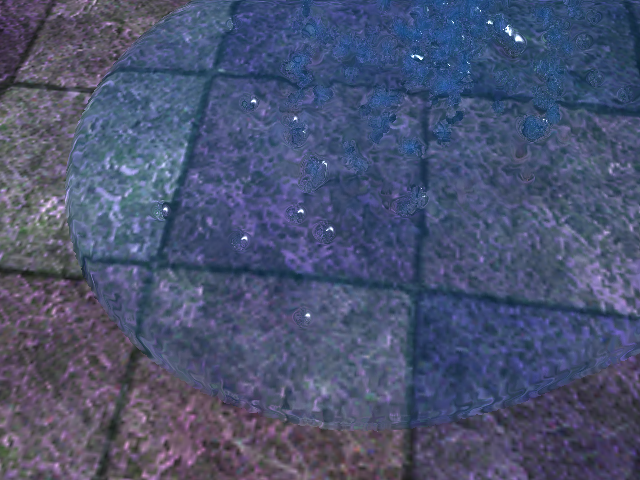
\includegraphics[width=1\textwidth]{gauss_fixed_far}
(b) Farther from camera
\end{minipage}
\caption{\textbf{Bilateral filtering results for different distances to camera} - The more distant fluid is from viewer the more smoothed its surface is. Also less edges are preserved due to z-buffer used resulting in more particles got blended into background surfaces. }
\label{edge_preservation}
\end{figure}
%\figuremacroW{edge_preservation}{Bilateral filtering results for different distances to camera}{The more distant fluid is from viewer the more smoothed its surface is. Also less edges are preserved due to z-buffer used resulting in more particles got blended into background surfaces}{0.7}

Another issue is that when using fixed kernel size filter. As particles are rendered smaller with the distance to the viewer further surfaces will be more smooth than closer surfaces (see figure~\ref{edge_preservation}). Solving that problem requires using filter with variable kernel size, depending on fragment distance from viewer. This is implemented using several precomputed kernels which are passed as array of 1D textures into shader. Section~\ref{sec:curvatureflowsmoothing} will describe another smoothing technique that doesn't suffer from this problem. 

\subsubsection{Curvature flow smoothing} \label{sec:curvatureflowsmoothing}
This technique was presented in \cite{laanSainz2009}. It utilizes curvature flow to smooth surface. Curvature is a differential geometry concept which measures how geometric object deviates from being flat. Curvature flow evolves surface by moving it's points with velocity given by:
\begin{equation}
\vec{v_p} = -\kappa_p \hat{n}_p
\end{equation}
where $\kappa_p$ is mean curvature at point $p$ and $\hat{n}_p$ is unit normal vector at point $p$.
We can then write equation of motion under mean curvature for surface $u$:
\begin{equation}
\label{eq:curvature_flow}
\frac{du}{dt} = -\kappa \vec{n}
\end{equation}
Since we are working with depth texture ($z(x, y)$) we only move surface in direction of $z$ axis. This allows to omit surface normal:
\begin{equation}
\label{eq:curvature_flow_z}
\frac{dz}{dt} = -\kappa
\end{equation}

In depth buffer, areas with highest curvature occurs in contact places of particles (see figure~\ref{sudden_changes}). Those are also areas that requires the most smoothing. Boundary conditions have to be enforced in equation~\ref{eq:curvature_flow} to ensure that different patches of fluid won't be blended together (see figure~\ref{sudden_changes}).

\figuremacroW{sudden_changes}{Depth texture in 2D}{Areas with highest curvature marked by green circles. In red circle there is area that shouldn't be smoothed.}{1.0}

Mean curvature is defined as:
\begin{equation} \label{eq:mean_curvature}
\kappa = \frac{1}{2} \triangledown \dot \hat{n}
\end{equation}

To compute surface normal from depth texture we need to invert perspective projection to obtain point P:
\begin{equation}
P(x, y) = 
\begin{pmatrix}
\frac{2x -1.0}{F_x} \\
\frac{2y -1.0}{F_y} \\
1
\end{pmatrix}
z(x,y) = 
\begin{pmatrix}
W_x \\
W_y \\
1
\end{pmatrix} z(x,y)
\end{equation}
where $F_x$ and $F_y$ is camera's focal length in the x and y direction. To compute surface normal we have to take cross product between partial derivatives of P in x and y directions:

\begin{align} \label{eq:surface_normal}
n(x, y) &=  \frac{\partial P}{\partial x} \times \frac{\partial P}{\partial y}  \nonumber \\
	&= 
		\begin{pmatrix} 
			C_x z  + W_x \frac{\partial z}{\partial x} \\
			W_y \frac{\partial z}{\partial x} \\
			\frac{\partial z}{\partial x}
		\end{pmatrix}
		\times
		\begin{pmatrix} 
			W_x \frac{\partial z}{\partial y} \\
			C_y z  + W_y \frac{\partial z}{\partial y} \\
			\frac{\partial z}{\partial y}
		\end{pmatrix} \nonumber \\		
	&\approx
		\begin{pmatrix}
			C_x z \\
			0 \\
			\frac{\partial z}{\partial x}
		\end{pmatrix}
		\times
		\begin{pmatrix}
			0 \\
			C_y z \\
			\frac{\partial z}{\partial y}
		\end{pmatrix}
		=
		\begin{pmatrix}
			-C_y \frac{\partial z}{\partial x} \\
			-C_x \frac{\partial z}{\partial y} \\
			-C_x  C_y z 
		\end{pmatrix} z
\end{align}
where $C_x = \frac{2}{F_x}$, $C_y = \frac{2}{F_y}$. \cite{laanSainz2009} suggested to discard terms of derivative of P that depend on view position $W_x$ and $W_y$. Unit normal is given by:
\begin{equation} \label{eq:view_space_normal}
	\hat{n} = \frac{n(x, y)}{|n(x, y)|} = \frac{\left(-C_y \frac{\partial z}{\partial x}, -C_x \frac{\partial z}{\partial y}, -C_x  C_y z\right)^T}{\sqrt{D}}
\end{equation}
in which
\begin{equation}
D = C^2_y \left(\frac{\partial z}{\partial x}\right)^2 + C^2_x \left(\frac{\partial z}{\partial y}\right)^2 + C^2_x  C^2_y z^2 
\end{equation}

Now $\hat{n}$ can be substituted into equation~\ref{eq:mean_curvature}. The z component of divergence will be 0 as $\frac{\partial z}{\partial z} = 0$. Thus we have:
\begin{equation}
\kappa = \frac{1}{2} \left( \frac{\partial \hat{n}}{\partial x} + \frac{\partial \hat{n}}{\partial y} \right) = \frac{C_y E_x + C_x E_y}{D^{\frac{3}{2}}}
\end{equation}
in which 
\begin{equation}
E_x = \frac{1}{2} \frac{\partial z}{\partial x} \frac{\partial D}{\partial x} - \frac{\partial^2 z}{\partial x^2}D
\end{equation}
\begin{equation}
E_y = \frac{1}{2} \frac{\partial z}{\partial y} \frac{\partial D}{\partial y} - \frac{\partial^2 z}{\partial y^2}D
\end{equation}

To modify z values in each iteration Euler integration of equation~\ref{eq:curvature_flow_z} is used. Amount of smoothing can be controlled by number of iterations - the more iterations the smoother surface will be. Since equation~\ref{eq:curvature_flow_z} is stiff, integration time step has to be very small to retain stability. If it is too large undesirable visual artifacts appears (figure~\ref{curvature_instabilities}). My experiments shown that time step should be less than $10^{-7}$.
\figuremacroW{curvature_instabilities}{Curvature flow smoothing artifacts}{artifacts occurs when integration time step is too big}{0.7}

\subsection{Thickness} \label{sec:thickness}
This step is performed to determine how opaque is surface in given point. It is done by rendering particles as circles into depth buffer with additive blending enabled. Resulting thickness texture is then smoothed with Gaussian filter (this time regular one). In order to speed up rendering process this texture can be rendered with lower resolution and then applied with linear interpolation. 

\subsection{Rendering} \label{sec:screenspace_rendering}
Last step assembles fluid surface with background image. As an input it takes smoothed fluid's depth texture, thickness texture and texture with rest of the scene rendered. 

First normal vectors have to be computed using finite differences of surface depth $d(x, y)$. This is done as in equation~\ref{eq:view_space_normal}. Finite differences are computed in one direction, except edges to avoid undesirable smoothing (figure TODO). 

Shading is done using Fresnel equation and a Phong specular highlight. Output color $C_{out}$ is given by:

\begin{equation}
\label{shading_equation}
C_{out} = a (1 - F(n \cdot v)) + b F(n \cdot v) + k_s (n \cdot h)^{\alpha}
\end{equation}

where $\alpha$ is refracted fluid color, $\beta$ is reflected color, $k_s$ and $\alpha$ are constants for Phong specular highlight, $n$ is a normal vector of the fluid surface, $v$ is view vector (from surface to camera), $h$ is the half vector between light vector and the view vector and $F(n \cdot v)$ is Fresnel function. 
$F(n \cdot v))$ is computed using Schlick's approximation:
\begin{equation}
F(n \cdot v)) = F_0 + (1 - R_0)(1 - n \cdot v)^5
\end{equation}
where $F_0$ is the value of reflectance when angle between normal vector and view vector is 0. 

Refracted fluid color $a$ is given by:
\begin{equation}
\label{refracted_color}
a = lerp(C_{fluid}, S(x + \beta n_x, y + \beta n_y), e^{-k T(x, y)})
\end{equation}
where $S(x, y)$ texture with rest of the scene, $\beta$ is the parameter which controls how much background scene is refracted, $C_fluid$ is the color of the fluid itself and $k$ is a given constant. As can be seen thickness texture is used to control fluid opacity - the thicker fluid is the less opaque it is. Refraction is approximated by sampling underlying scene texture $S(x, y)$ with texture coordinates perturbed by normal of the surface. Amount of perturbation is controlled by $\beta$ parameter which depends on thickness:
\begin{equation}
\beta = T(x, y) \gamma
\end{equation}
where $\gamma$ is a constant which depends on the kind of fluid. 

Reflected color $b$ is computed using environmental mapping. 

\section{Isosurface extraction} \label{sec:isosurfaceextraction}
Classic algorithm for isosurface extraction is marching cubes (see \cite{LorensenCline1987}). It takes 3d array with scalar field values as an input and produces list of triangles. Algorithm divides space into cubes, and proceeds through scalar field taking one cube at a time (each cube consists of 8 vertices with scalar field values). Field value at each cube vertex is tested to be above or under given threshold and then appropriate triangle configuration is taken from lookup table (there are 256 triangle configurations).

This method is not suitable for extraction surface from particles. Firstly scalar field values at cube corners are not given. Secondly visiting each cube is not efficient as most of cubes doesn't contain surface. Several variations of marching cube algorithm were created to overcome those problems. The algorithm used is a multithreaded version of the one presented in \cite{RosenbergBirdwell2008}. This is a surface following version of marching cubes with a fast particle lookup cache technique. 

\subsection{Overview} \label{sec:iso_overview}
Algorithm takes as an input a list of particles positions, particle's radius of influence ($R_c$), isosurface threshold and produces list of triangles. Particle's radius of influence is something different than particle size (or simply particle radius - $R$), because its value is usually greater. Every particle produces a field that has non-zero values within $R_c$ from particle center. The field value in given point of space $p$ is a sum of field values generated by all particles within $R_c$. This can be represented by:
\begin{equation}
\label{eq:field_equation}
F(p) = \sum_{s~\epsilon~S_{R_c}(p)} f(dst(s, p))
\end{equation}
where $s$ is a center of particle, $S_{R_c}(p)$ is a sphere with $p$ as a center and radius of $R_c$. $f(r)$ is a field function of single particle. It can be any function that is radially monotonic, continuous and has non-zero values within $R_c$ from particle center. Following function is often used as it can be computed efficiently using few operations:
\begin{equation}
\label{eq:single_field_equation}
f(r) = \left\{ \begin{array}{ll}
({r \over \sqrt{2}R_c} )^4 - ( {r \over \sqrt{2}R_c} )^2 + 0.25 & \textrm{if $r < R_c$}\\
0 & \textrm{otherwise}\\
\end{array} \right.
\end{equation}

When $R_c > R$ neighboring particles combines into one smooth surface  (figure~\ref{metaballs}). This is a common technique known as metaballs \cite{Blinn1982}. The biggest problem here is to efficiently compute field values at corners and to traverse space in the most optimal way. Those topics will be described in following subsections.

\begin{figure}[ht]
\begin{minipage}[b]{0.24\linewidth}
\centering
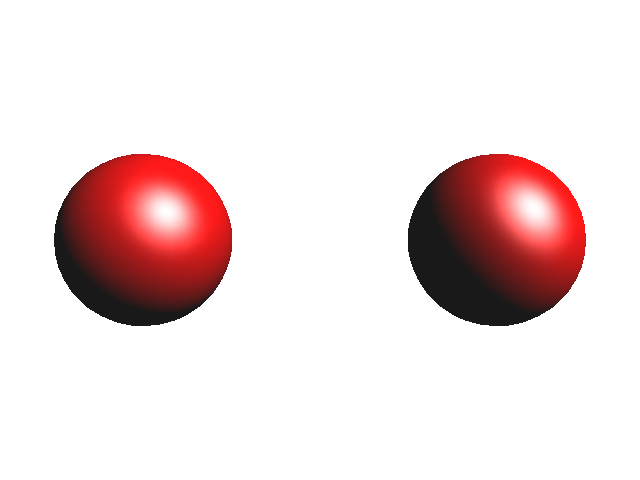
\includegraphics[width=1\textwidth]{meta1}
Step 1
\end{minipage}
\begin{minipage}[b]{0.24\linewidth}
\centering
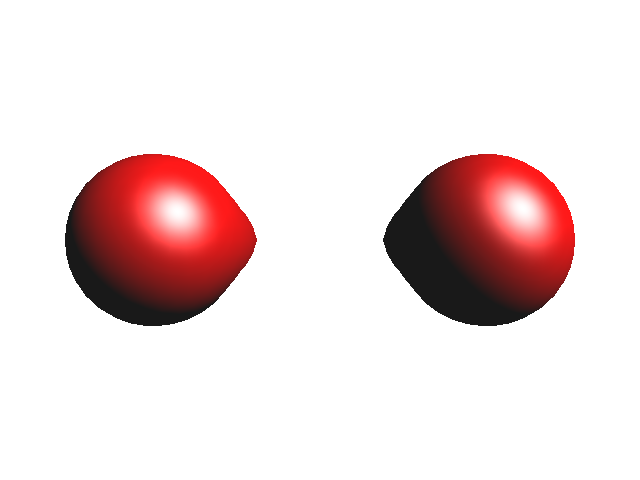
\includegraphics[width=1\textwidth]{meta2}
Step 2
\end{minipage}
\begin{minipage}[b]{0.24\linewidth}
\centering
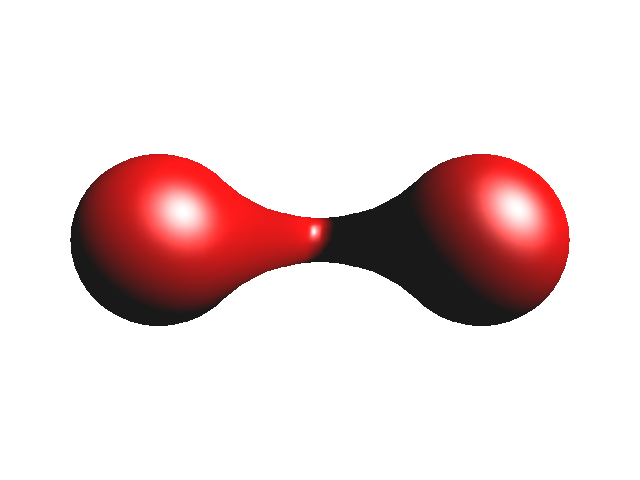
\includegraphics[width=1\textwidth]{meta3}
Step 3
\end{minipage}
\begin{minipage}[b]{0.24\linewidth}
\centering
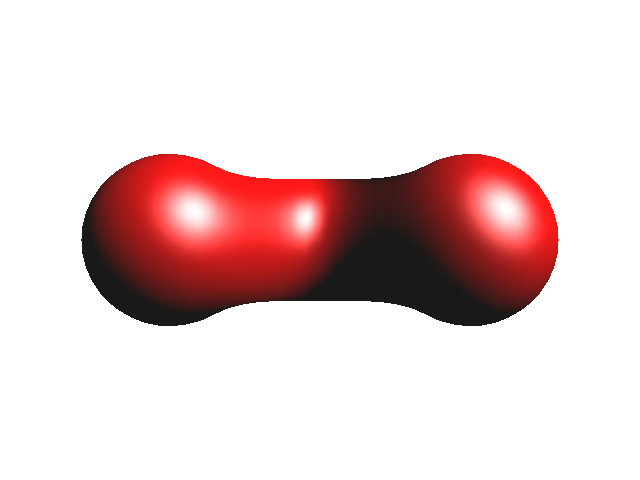
\includegraphics[width=1\textwidth]{meta4}
Step 4
\end{minipage}
\begin{minipage}[b]{0.24\linewidth}
\centering
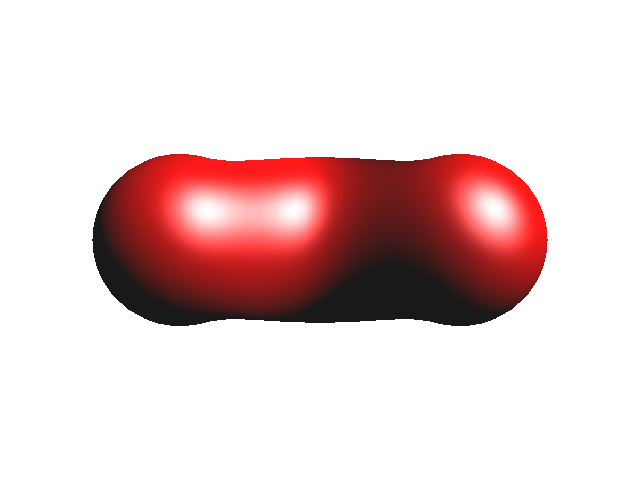
\includegraphics[width=1\textwidth]{meta5}
Step 5
\end{minipage}
\begin{minipage}[b]{0.24\linewidth}
\centering
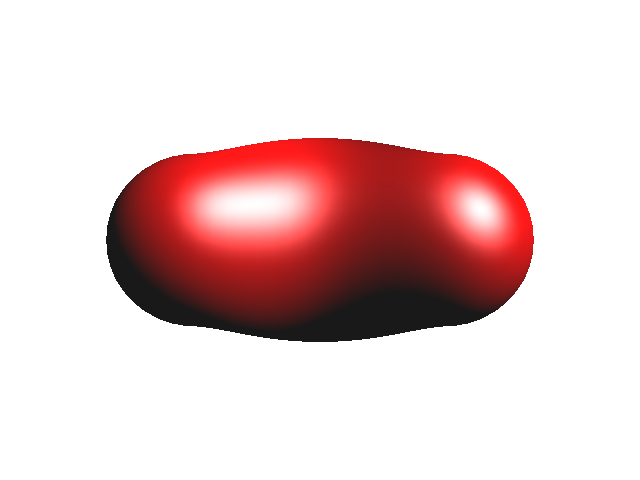
\includegraphics[width=1\textwidth]{meta6}
Step 6
\end{minipage}
\begin{minipage}[b]{0.24\linewidth}
\centering
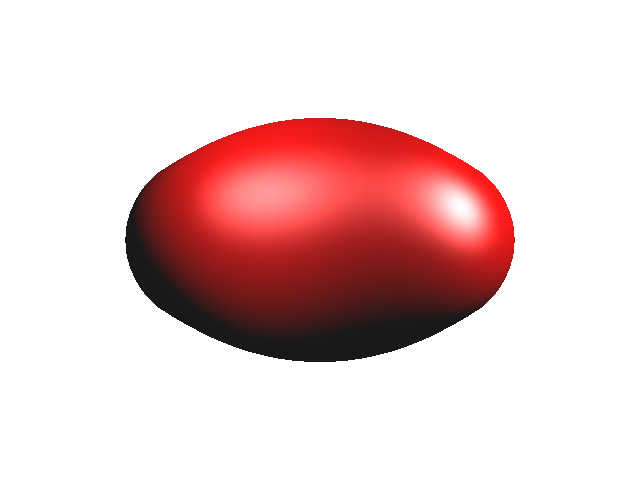
\includegraphics[width=1\textwidth]{meta7}
Step 7
\end{minipage}
\begin{minipage}[b]{0.24\linewidth}
\centering
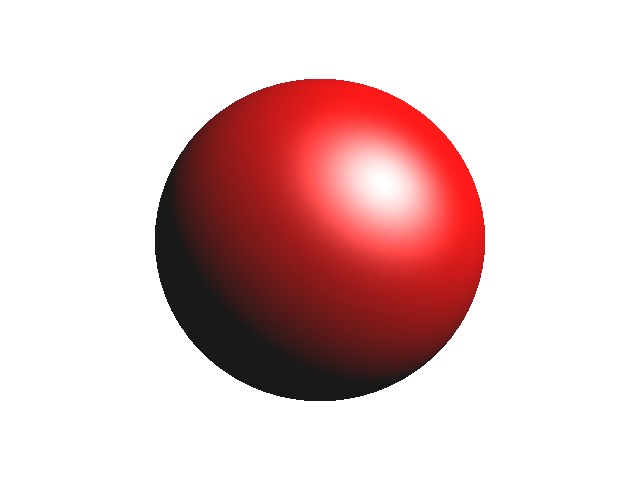
\includegraphics[width=1\textwidth]{meta8}
Step 8
\end{minipage}
\caption{\textbf{Metaballs} - illustrates how particles combines into one surface as their approach closer and closer together. }
\label{metaballs}
\end{figure}

\subsection{Block subdivision} \label{sec:block_subdivision}
Space is divided into blocks containing cubes (figure~\ref{block_subdivision}). Such division aims for:
\begin{itemize}
\item Reduce memory consumption - smaller blocks contains less particles and cubes. 
\item Allowing easy way of parallelization of algorithm - because processing one block is independent of processing other blocks. 
\end{itemize}
Blocks are expanded to contain also particles that lies outside them but may influence the field values inside block. That means the block must also contain particles lying within $R_c$ distance from it - this area is called margin and has special treatment, which will be described in next section. Expanding blocks makes parallel processing very easy as dependencies between block disappear.

\figuremacroW{block_subdivision}{Block subdivision}{space is divided into blocks which overlaps. Each block is divided into cubes of size S.  Image taken from~\cite{RosenbergBirdwell2008}}{0.7}

Block subdivision is a first step of the algorithm. For every particle containing blocks are determined. One particle can be contained in at most 8 blocks due to blocks overlapping. Each block has a list of particles lying within its boundary. 

\subsection{Block processing} \label{sec:block_processing}
Processing of block starts from building a particle lookup cache which will be described in section \ref{sec:lookupcache}. Next, surface following marching cube algorithm is run inside block. The algorithm is named \textit{marching slices} in \cite{RosenbergBirdwell2008}. Block containing $n \times n \times n$ cubes is divided to n slabs and n+1 slices (figure~\ref{block_image}). Division is made in parallel to XY plane. Each slab contains $n \times n \times 1$ cubes and each slice contains $(n+1) \times (n+1) \times 1$ cube corners. Slices lies between slabs and serves as a cache for field values computed at corners. In addition neighboring slabs share slices that lies between them. Each slab has a list of cubes, lying within it, that should be visited - a \textit{todo list}.

\figuremacroW{block_image}{Structure of a block.  Image taken from~\cite{RosenbergBirdwell2008}}{}{1.0}

To speed up a marching cubes algorithm we would like to traverse only cubes that contains surface. This requires finding so called \textit{seed cubes} - initial cubes at which algorithm will start traversing block. We then choose one of the slabs that contains one or more seed cubes and pick up one cube. Field values at cube corners are calculated and put into slice caches, surface is polygonized and neighboring cubes that contain surface are added to a \textit{todo lists} of corresponding slabs. 

If we picked up a random slabs and cubes each time then we would have to keep all cached values in slices while processing a cube. The idea of marching slices is to decrease memory, that cache consumes, by traversing cubes slice by slice and deallocate caches as soon as possible. This can be done by always picking the lowest slab with not empty \textit{todo list} and finding seeding cubes in the lowest possible slabs. 

The optimum for finding seed cubes would be to find surface's all local minimas - then we would only have to store cache in slices below and above current slab. However this approach would be time consuming. \cite{RosenbergBirdwell2008} used heuristic approach with complexity O(P) where P is a number of particles. The algorithm is as follows:
\begin{verbatim}
for every particle:
        take a corner closest to particle center
        while F(c) > treshold and |c - c_start| < 2 do
                c = corner below c
        if F(c) < treshold
                add cube to it's slab todo list
\end{verbatim}

This method will not find local minimas every time as it always goes down from the center of a particle (see figure~\ref{fig_local_minima}).

\figuremacroW{fig_local_minima}{Finding local minimum}{In this example algorithm fails to find local minimum. We have two particles forming metaball. Seeding cubes and paths to find them are marked blue, actual local minimum is marked in red circle}{0.7}

\subsection{Lookup cache}\label{sec:lookupcache}
To compute field value for a given corner all particles that lies within $r_c$ from it has to be found. This task can be accomplished by building space partitioning data structure like octtree or kdtree \cite{Bentley1975}. However costs of building spatial data structures are relatively high, and the nearest neighbor finding algorithm requires floating point computations. \cite{RosenbergBirdwell2008} presented another way to accomplish this task. Presented method uses only integer comparison. The main observation is that we are looking nearest particles in discrete points. Thus obvious approach would be to create a linked list for every corner containing all particles lying within $r_c$ from it. So for every particle we would traverse all corners lying inside a sphere of radius $r_c$ and update their particles list by inserting the current one.  The main disadvantage of this approach is that we would have to store that information for each corner, and for every corner we would have to store a separate list. This can be improved by using more sparse data structure. For a block we can store only one slice (so called projection slice) as a 2D array of $N+1$ by $N+1$. Element (x, y) of the array represents a column (x, y) of corners and stores a linked list of particles that have an influence in that column (figure~\ref{particle_lookup_cache}). To make particle lookup procedure more efficient each list is sorted by particles z coordinate. Each element of the list contains three integer values - $min_z$, $max_z$, $mid_z$ and a pointer to particle. $min_z$ and $max_z$ specifies range of slices in which particle has influence and $mid_z$ is a slab that contains center of the particle. 

\figuremacroW{particle_lookup_cache}{Particle lookup cache}{Each cell of projection slice represents a column in block and stores linked list of particles that have influence in that column. Image taken from~\cite{RosenbergBirdwell2008}}{0.7}

Initialization of cache starts with sorting all particles by z coordinate. Then we iterate over sorted particles and each particle is inserted into all columns in which it has an influence. 

To lookup particles that have influence in given corner at location (x, y, z) we have to check all columns from projection slice that lies within $R_c$ radius from that corner. This narrows search to cylinder of radius $\left \lceil \frac{R_c}{S} \right \rceil$ and height equal to height of block. Next each column is iterated from begin to search for first element ($E_f$) with $mid_z \geq z - \left \lceil \frac{R_c}{S} \right \rceil$. Then iteration is continued until topmost element ($E_l$) with $mid_z \leq  z + \left \lceil \frac{R_c}{S} \right \rceil$. This narrows height of searching cylinder to $2R_c$. In order to further narrow this into sphere of radius $R_c$  every element between $E_f$ and $E_l$ is tested for having $min_z \leq z$ and $max_z \geq z$. Such a procedure return only particles that have influence in given corner. 

Further discussion concerning performance and memory consumption of this lookup technique can be found in \cite{RosenbergBirdwell2008}. Authors also provide comparison with other lookup methods. 

\subsection{Normals generation}\label{sec:normals}
In order to properly shade extracted surface normal vectors have to be computed for each vertex. The simplest approach is to generate one normal for each triangle, perpendicular to its surface and assign it to all three triangle vertices. This requires that vertices are not shared between triangles thus it's not applicable with surface extraction method used. 

Another approach is to compute normals at corners of a grid as a gradient of scalar field: 
\begin{equation}
	\vec{n}_{i,j,k} = 
	\begin{bmatrix}
		\frac{F_{i-1, j, k} - F_{i+1, j, k}}{W}\\	
		\frac{F_{i, j-1, k} - F_{i, j+1, k}}{H}\\	
		\frac{F_{i, j, k-1} - F_{i, j, k+1}}{D}
	\end{bmatrix}
\end{equation}
where W, H and D are dimensions of cube, $\vec{n}_{i, j, k}$ is normal at corner (i, j, k) and $F_{i, j, k}$ is value of scalar field at corner (i, j, k).
As values of field are given only at corners and vertices in most cases lies between them the interpolation is required. Also this increases amount of corners at which scalar field value must be computed. Another disadvantage is that in order to speed up process of normal generation in this case, normals can't be generated after extracting isosurface. This is due to clearing caches, and thus normals have to be computed in the same time vertex are added to \textit{todo list}. This results in more complicated code.

Yet another approach is to compute normal for every triangle that includes given vertex and take an average or weighted average as a vertex normal. Simple average can be computed effectively however it produces visible artifacts for sparse grids. This is because some triangles are long and narrow and should not have so much impact on final normal. To solve this weighted average can be used. Weights can be the area of triangle or an angle by given vertex. 

\figuremacro{fig_normal_approx}{Normal vector computation for corner}{ $ \vec{n} = f(|\vec{v1}|) \frac{\vec{v1}}{|\vec{v1}|} +  f(|\vec{v2}|) \frac{\vec{v2}}{|\vec{v2}|}$}

As approximating surface normal at given vertex as weighted average of adjacent triangles normals doesn't give satisfying results I have used different approach. It is illustrated on figure~\ref{fig_normal_approx}. For every visited corner normal vector is computed as a weighted average of vectors pointing from particle centers to this corner. The weights are field values generated by each particle in this corner. When vertex is generated between corners normal vector is computed as weighted average of corners normals. Figure~\ref{normal_generation} shows comparison between two last normal generation algorithms

\begin{figure}[ht]
\begin{minipage}[t]{0.5\linewidth}
\centering
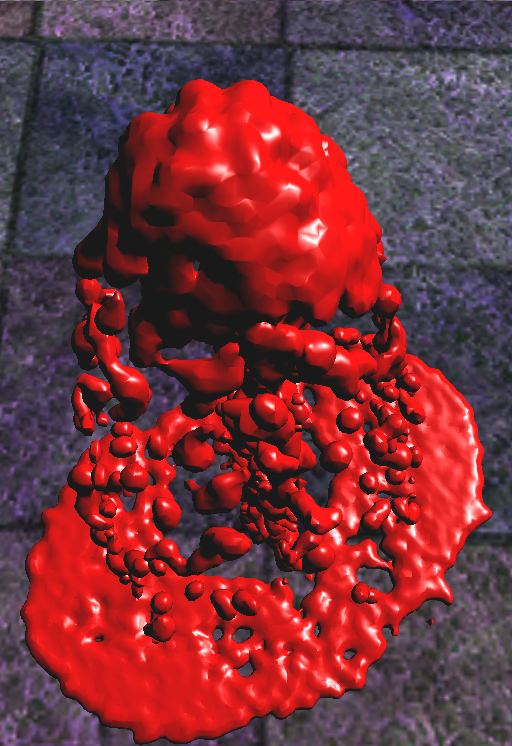
\includegraphics[width=1\textwidth]{normal_vec_cross}
(a) Weighted average based on length
\end{minipage}
\hspace{0.5cm}
\begin{minipage}[t]{0.5\linewidth}
\centering
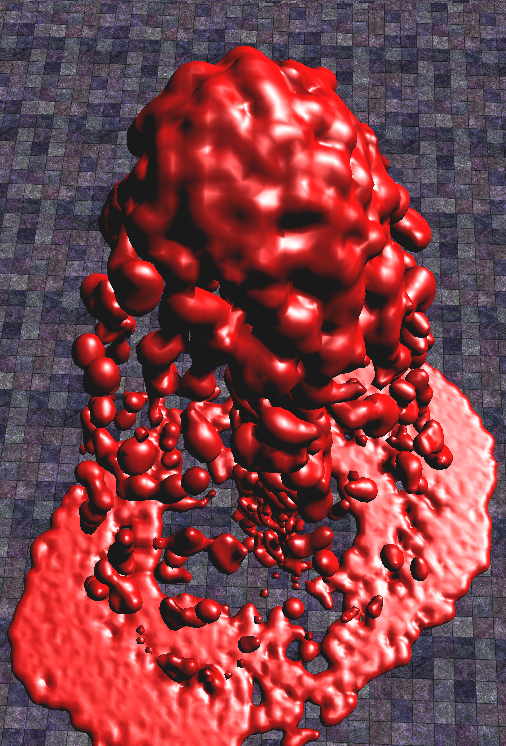
\includegraphics[width=1\textwidth]{normal_vec_improved}
(b) Vectors computed at each visited corner
\end{minipage}
\caption{\textbf{Comparison of normal generation techniques} - (a) - weighted average of normals of adjacent triangles, (b) - weighted average of normals computed for corners. }
\label{normal_generation}
\end{figure}

\subsection{Multithreading}
\cite{RosenbergBirdwell2008} presented algorithm that runs in one thread. However algorithm has a potential of parallelization due to independence of block processing. Parallelization of this algorithm is even more desired as nowadays CPU manufacturers increase performance by multiplying CPU cores instead of increasing clock frequency of a single core. 

As mentioned before processing of block is independent of one another. The algorithm uses thread pool which size can be configured and the single task is a single block. The architecture is illustrated on figure~\ref{threading_architecture}. The single thread checks if there are still blocks to process in blocks queue, takes one and extracts surface in this block. Result of extracting surface in one block is put into results list. Thread stops when there are no more task in queue. As the main thread doesn't take part in surface extraction there is possibility of working asynchronously. Main thread can render surface extracted in previous frame while working threads are extracting surface for the current frame.

\figuremacroW{threading_architecture}{Threading architecture}{architecture diagram of parallelization of surface extraction algorithm}{0.7}

\subsection{Rendering}
Rendering fluid as a mesh is a simpler task since we already have surface and normals. Only one problem arises when fluid has to be rendered with opacity. Traditionally it would require rendering graphic primitives in back to front order with alpha blending enabled. However algorithm used for surface extraction doesn't produce primitives in such order.  \cite{RosenbergBirdwell2008} noted that this algorithm can be transformed to produce primitives with desired ordering. Since this modification produces some extra overhead I used different approach - similar to one used in section \ref{sec:screenspace_rendering}.

First background scene is rendered into texture $S(x, y)$. Then when fluid meshes are rendered this texture is sampled with texture coordinates perturbed using normals of the surface. This computation is done in fragment shader. As scene texture cannot be applied to meshes itself but it should be applied to the whole screen texture coordinates are computed in fragment shader based on screen coordinates of fragment:
\begin{equation}
(x, y) = (\frac{p_x}{width}, \frac{p_y}{height})
\end{equation}
where $(p_x, p_y)$ are screen coordinates of fragment, $width$ and $height$ are dimensions of the screen. 
% ---------------------------------------------------------------------------
% ----------------------- end of thesis sub-document ------------------------
% ---------------------------------------------------------------------------